%%%%%%%%%%%%%%%%%%%%%%%%%%%%%%%%%%%%%%%%%%%%%%%%%%%%%%%%%%%%%%%
%
% Welcome to Overleaf --- just edit your LaTeX on the left,
% and we'll compile it for you on the right. If you open the
% 'Share' menu, you can invite other users to edit at the same
% time. See www.overleaf.com/learn for more info. Enjoy!
%
% Note: you can export the pdf to see the result at full
% resolution.
%
%%%%%%%%%%%%%%%%%%%%%%%%%%%%%%%%%%%%%%%%%%%%%%%%%%%%%%%%%%%%%%%
\documentclass{article}
\usepackage{tikz}
\usepackage{verbatim}

\begin{comment}
:Title: Intersecting lines
:Tags: Axes, Basics, Coordinate systems

An example of using the intersection coordinate systems. Both the ``intersection`` and 
``perpendicular`` coordinate system are used. The latter is a special case of the former,
but has the shorter and more convenient ``-|`` and ``|-`` syntax. 

\end{comment}

\begin{document}

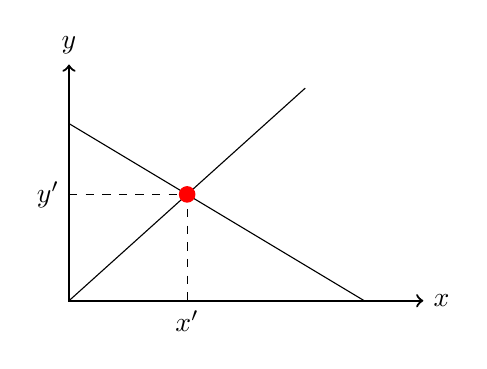
\begin{tikzpicture}[scale=1.5]
    % Draw axes
    \draw [<->,thick] (0,2) node (yaxis) [above] {$y$}
        |- (3,0) node (xaxis) [right] {$x$};
    % Draw two intersecting lines
    \draw (0,0) coordinate (a_1) -- (2,1.8) coordinate (a_2);
    \draw (0,1.5) coordinate (b_1) -- (2.5,0) coordinate (b_2);
    % Calculate the intersection of the lines a_1 -- a_2 and b_1 -- b_2
    % and store the coordinate in c.
    \coordinate (c) at (intersection of a_1--a_2 and b_1--b_2);
    % Draw lines indicating intersection with y and x axis. Here we use
    % the perpendicular coordinate system
    \draw[dashed] (yaxis |- c) node[left] {$y'$}
        -| (xaxis -| c) node[below] {$x'$};
    % Draw a dot to indicate intersection point
    \fill[red] (c) circle (2pt);
\end{tikzpicture}
\end{document}